\documentclass[10pt,a4paper]{article}
\usepackage[utf8]{inputenc}\usepackage[T1]{fontenc}\usepackage[brazil]{babel}
\usepackage{geometry,graphicx,amsmath,booktabs,microtype}
\geometry{margin=1.65cm}\setlength{\parindent}{0pt}\setlength{\parskip}{3pt}
\title{\vspace{-1em}\textbf{Identificação temporal de estados operacionais}\\\large Projeto 2 — Modelo Markoviano Oculto}
\author{Portfólio de Inteligência Artificial 1}\date{}
\begin{document}\maketitle\vspace{-1em}
\textbf{Resumo.} Um HMM discreto identifica estados industriais não observáveis a partir de padrões discretizados de sensores. Foram implementados Forward escalonado, Viterbi em logaritmos e Baum–Welch para estimação de parâmetros.
\section{Problema e modelagem}
Os estados ocultos são normal, sobrecarga, desgaste, pré-falha e falha crítica. Cada instante emite um de seis símbolos que representam combinações de vibração, temperatura e consumo. A matriz de transição é persistente: estados vizinhos são mais prováveis e a falha crítica é absorvente em 86\%. Essa hipótese representa degradação gradual, mas permite recuperação parcial.
\section{Métodos}
Com $A_{ij}=P(S_t=j\mid S_{t-1}=i)$, $B_{jk}=P(O_t=k\mid S_t=j)$ e $\pi_i=P(S_1=i)$, o Forward usa
\[
\alpha_t(j)=B_{j,o_t}\sum_i\alpha_{t-1}(i)A_{ij}.
\]
Após cada passo, $\alpha_t$ é dividido por sua soma; a log-verossimilhança é a soma dos logaritmos desses fatores. O Viterbi maximiza a mesma recorrência no domínio log e guarda retroponteiros. Baum–Welch alterna responsabilidades $\gamma$ e $\xi$ para atualizar $A$, $B$ e $\pi$ por EM, sem depender de biblioteca de HMM.
\section{Experimentos e resultados}
Uma sequência de 180 instantes foi gerada com semente 19 a partir do próprio modelo. O Viterbi obteve acurácia $0,856$ e F1 macro $0,740$. A matriz de confusão foi
\[
\begin{pmatrix}41&2&0&0&0\\5&29&2&0&0\\1&7&2&3&0\\0&0&1&21&4\\0&0&0&1&61\end{pmatrix}.
\]
\begin{figure}[h]\centering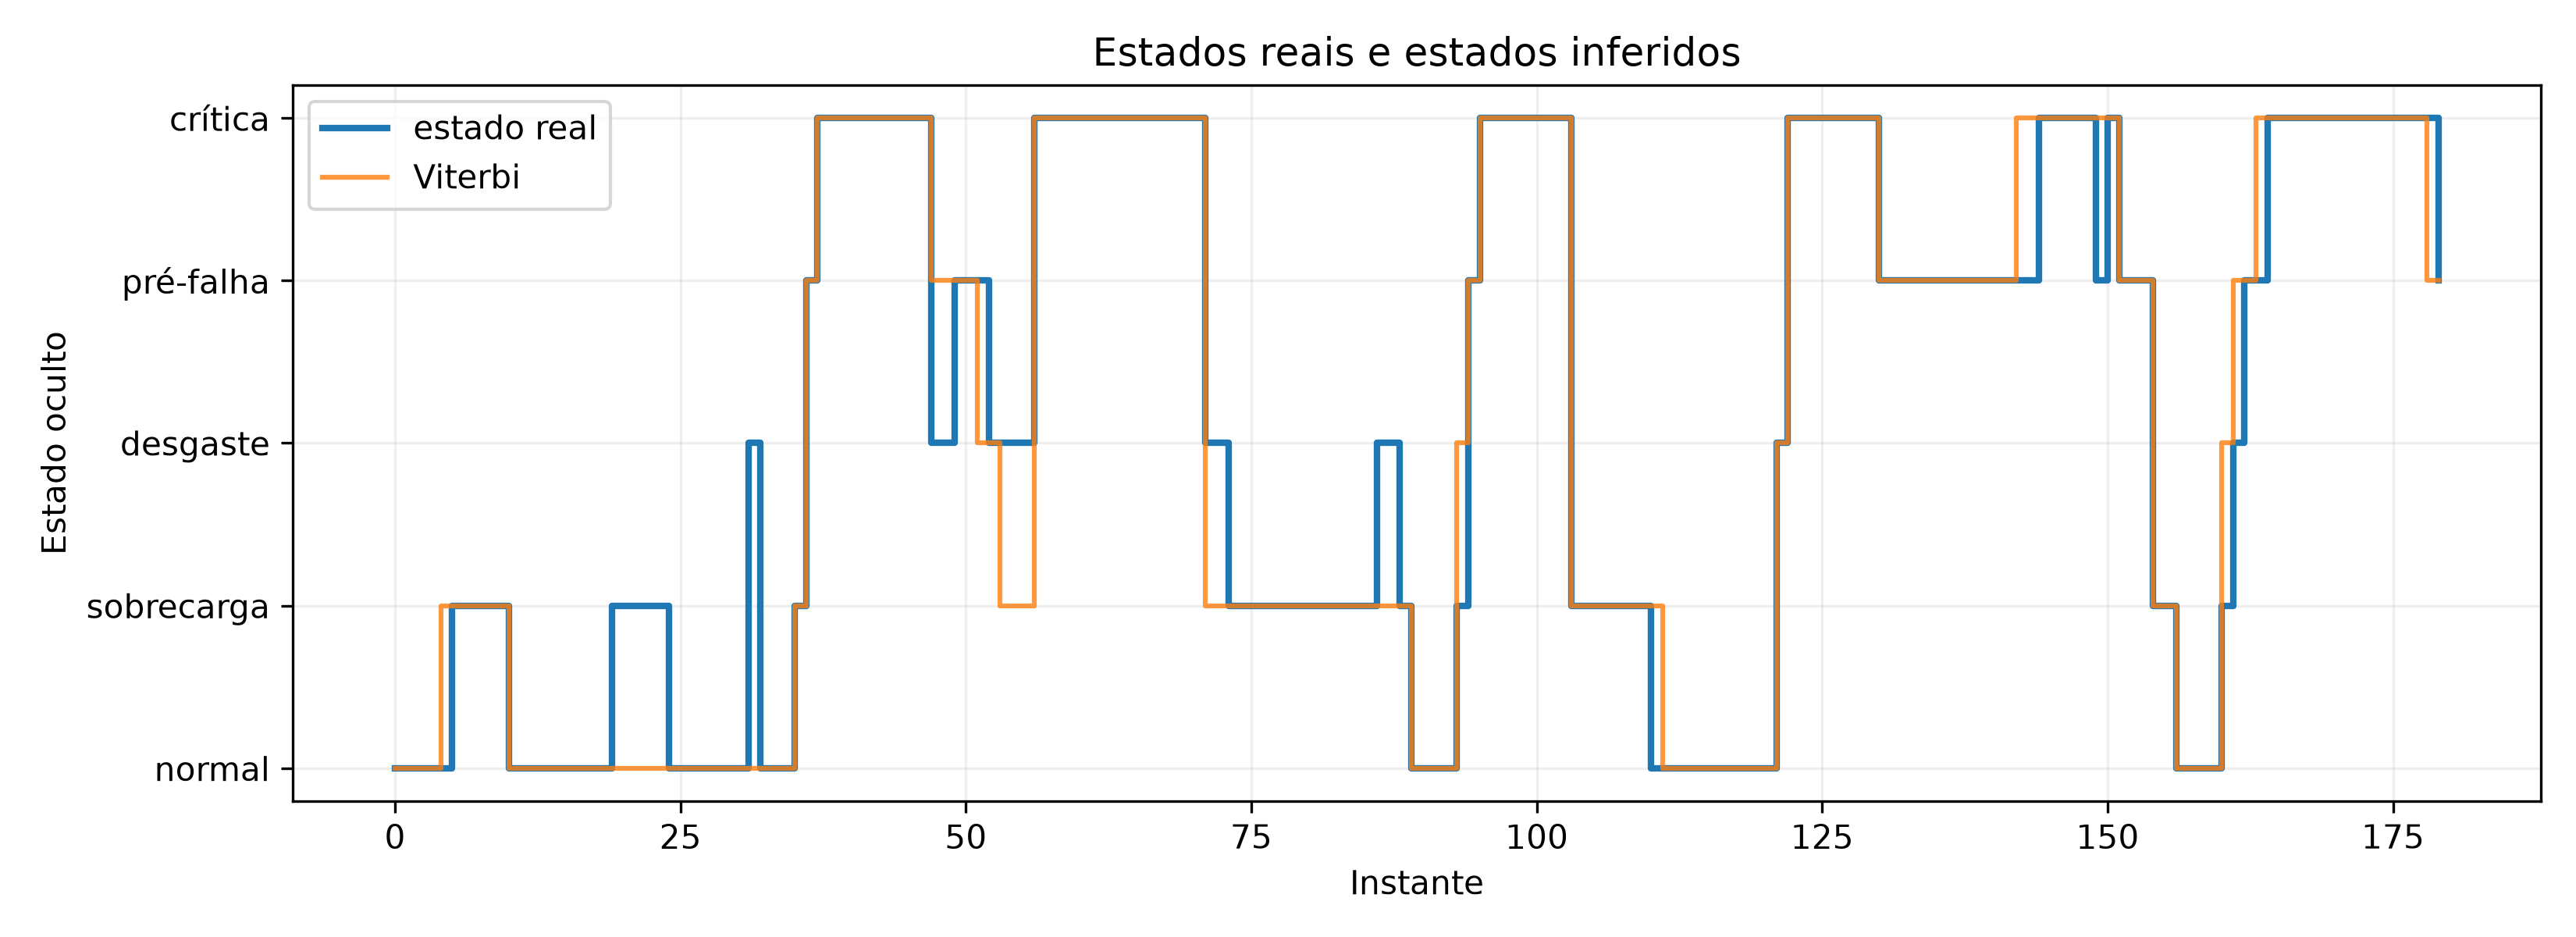
\includegraphics[width=.92\linewidth]{results/state_comparison.png}\caption{Estados reais e estimados.}\end{figure}
\begin{figure}[h]\centering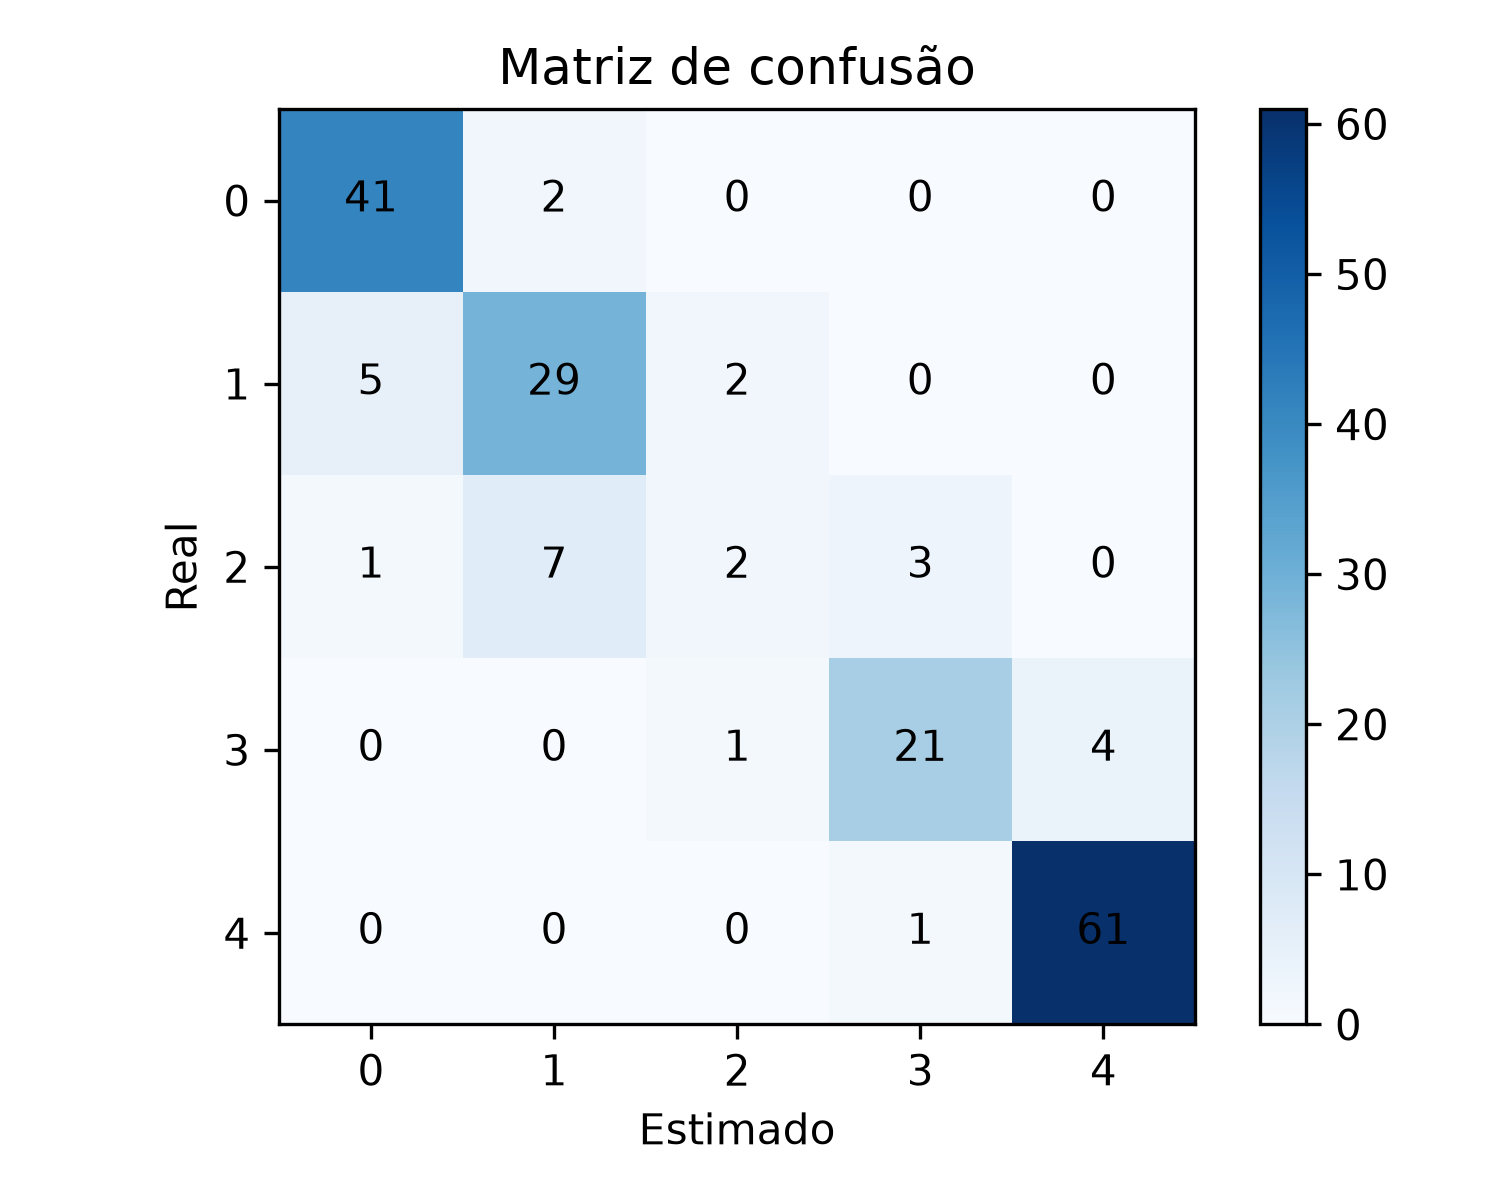
\includegraphics[width=.38\linewidth]{results/confusion_matrix.png}\hspace{.05\linewidth}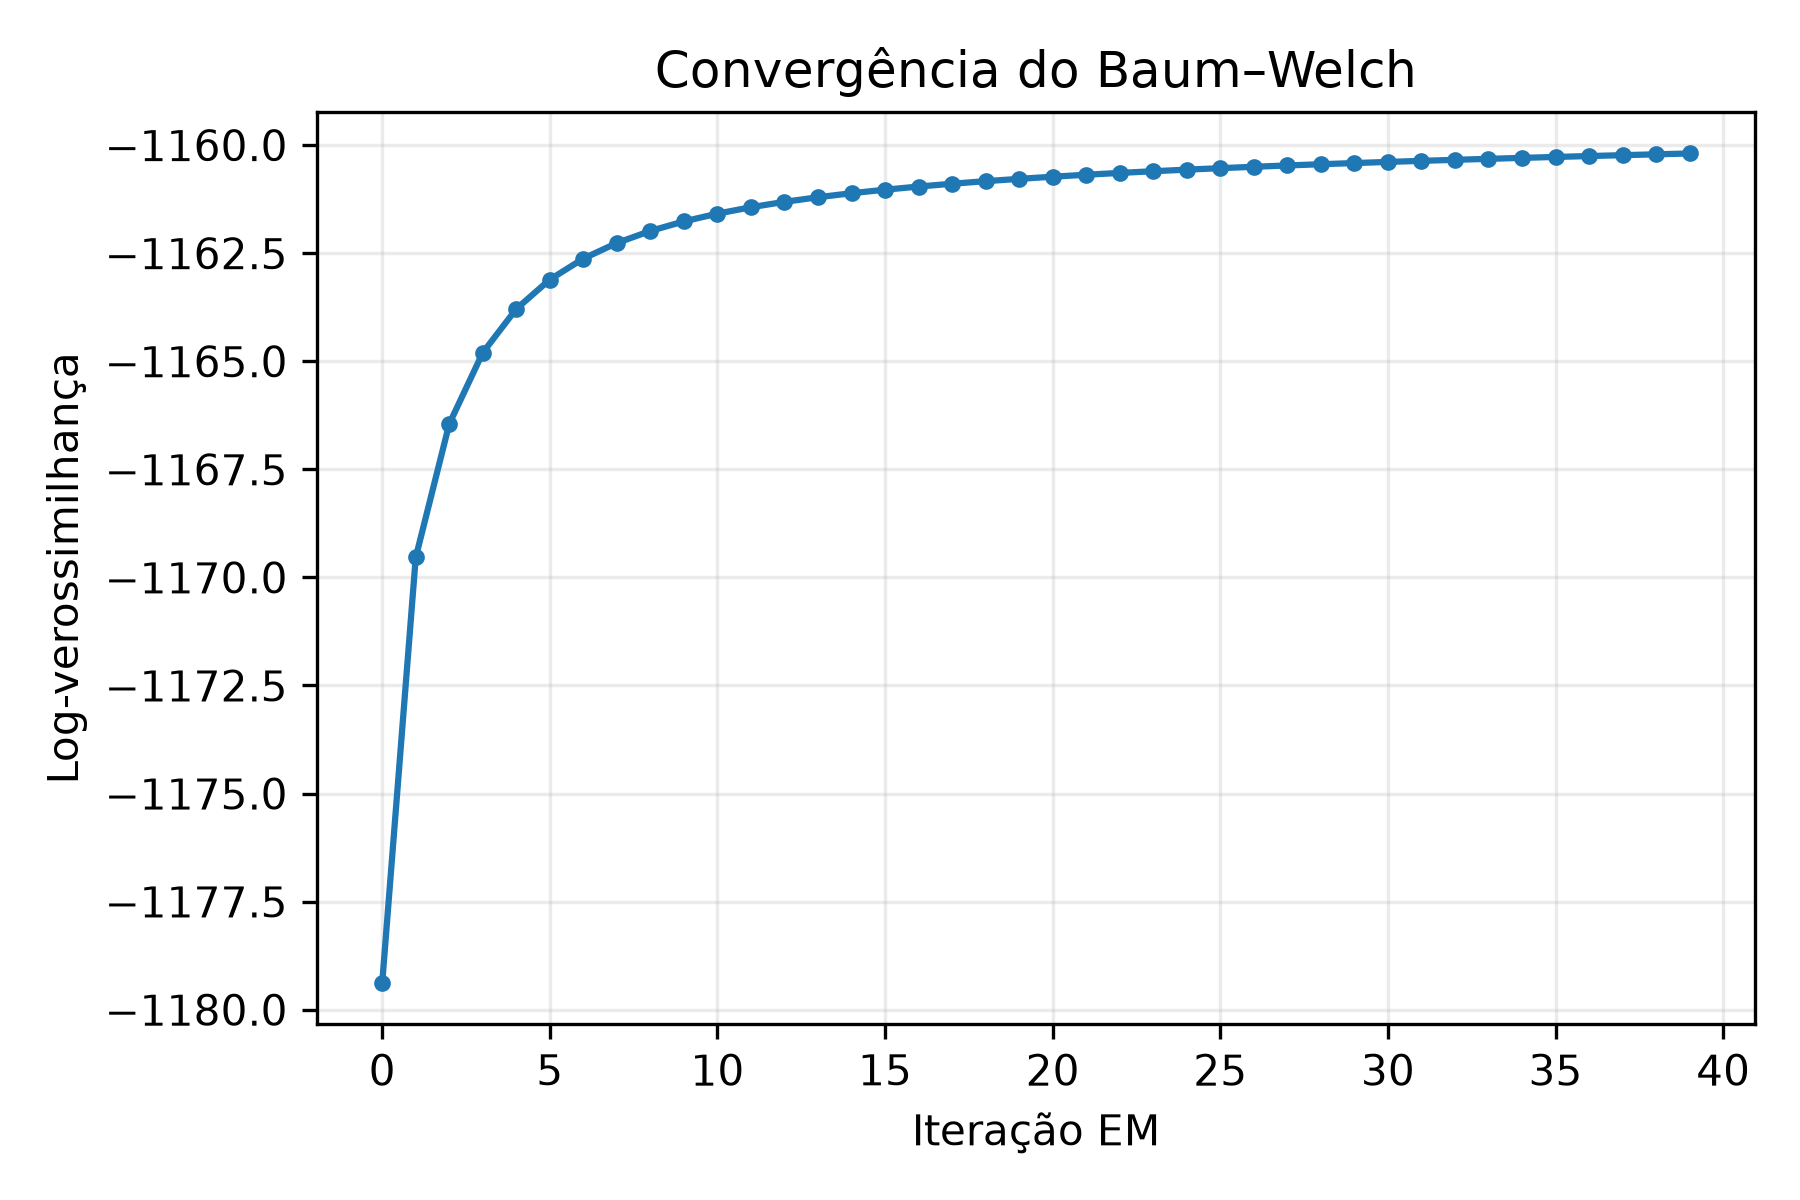
\includegraphics[width=.48\linewidth]{results/likelihood_analysis.png}\caption{Confusão e convergência do Baum–Welch.}\end{figure}
Em oito sequências adicionais de 100 símbolos, Baum–Welch aumentou a log-verossimilhança de $-1179,383$ para $-1160,193$ em 40 iterações. Os erros concentram-se em estados vizinhos, especialmente desgaste, comportamento esperado quando as emissões se sobrepõem.
\section{Conclusão}
O HMM recupera a dinâmica latente e produz alarmes temporais menos sensíveis a uma medição isolada. A identificação depende de separação das emissões e da hipótese de Markov de primeira ordem; mudanças abruptas, estados não modelados e parâmetros mal calibrados podem causar confusão. O escalonamento evita underflow em sequências longas. Referências: Rabiner (1989); Baum et al. (1970).
\end{document}
